%% LyX 2.2.3 created this file.  For more info, see http://www.lyx.org/.
%% Do not edit unless you really know what you are doing.
\documentclass[oneside,english]{extbook}
\usepackage{lmodern}
\renewcommand{\sfdefault}{lmss}
\renewcommand{\ttdefault}{lmtt}
\usepackage[T1]{fontenc}
\usepackage[latin9]{inputenc}
\usepackage{geometry}
\geometry{verbose,tmargin=25mm,bmargin=25mm,lmargin=25mm,rmargin=25mm}
\pagestyle{plain}
\setcounter{secnumdepth}{3}
\setcounter{tocdepth}{3}
\setlength{\parindent}{0bp}
\usepackage{babel}
\usepackage{float}
\usepackage{graphicx}
\usepackage{setspace}
\onehalfspacing
\usepackage[unicode=true,pdfusetitle,
 bookmarks=true,bookmarksnumbered=false,bookmarksopen=false,
 breaklinks=false,pdfborder={0 0 1},backref=false,colorlinks=false]
 {hyperref}

\makeatletter
%%%%%%%%%%%%%%%%%%%%%%%%%%%%%% User specified LaTeX commands.
\usepackage{amssymb}
\usepackage{color}
\usepackage{listings}
\definecolor{hellgelb}{rgb}{1,1,0.85}
\definecolor{colKeys}{rgb}{0,0,1}
\definecolor{colIdentifier}{rgb}{0,0,0}
\definecolor{colComments}{rgb}{1,0,0}
\definecolor{colString}{rgb}{0,0.5,0}
\lstset{
      language=Matlab,
      float=hbp,
      basicstyle=\footnotesize\ttfamily,
      identifierstyle=\color{colIdentifier},
      keywordstyle=\color{colKeys},
      stringstyle=\color{colString},
      commentstyle=\itshape\color{colComments},
      columns=fixed,
      tabsize=4,
      frame=single,
      framerule=1pt,
      extendedchars=true,
      showspaces=false,
      showstringspaces=false,
      numbers=left,
      numberstyle=\tiny\ttfamily,
      numbersep=1em,
      breaklines=true,
      breakindent=10pt,
      backgroundcolor=\color{hellgelb},
      breakautoindent=true,
      captionpos=t,
      xleftmargin=1em,
      xrightmargin=\fboxsep
}
\usepackage{lscape}
\usepackage{amsmath}
\usepackage{mathtools}
\usepackage{pifont}
\usepackage{color}
\usepackage{accents}

\delimitershortfall=-1pt
\let\Right\right
\let\Left\left
\makeatletter
\def\right#1{\Right#1\@ifnextchar){\!\right}{}}
\def\left#1{\Left#1\@ifnextchar({\!\left}{}}
\newcommand{\mathleft}{\@fleqntrue\@mathmargin0pt}
\newcommand{\mathcenter}{\@fleqnfalse}
\makeatother

\makeatother

\begin{document}
\renewcommand{\chaptername}{}
\renewcommand{\thechapter}{}
\pagenumbering{gobble}

\section*{THE EXTENDED KALMAN FILTER}

\begin{gather*}
\vec{x}_t \, = \, g\left(\vec{x}_{t-1},\, \vec{u}_t\right)\\\\
\begin{pmatrix*}[l]
x_t\,=\,g_1\left(x_{t-1},\,\vec{u}_t\right)\,=\, x_{t-1}\,+\,\left(Rs_t \,+\,\dfrac{W}{2}\right)\left(+\,\sin\left(\theta_{t-1}\,+\,\alpha_t\right)\,-\,\sin\left(\theta_{t-1}\right)\right)&\\
y_t\,=\,g_2\left(y_{t-1},\,\vec{u}_t\right)\,=\,y_{t-1}\,+\,\left(Rs_t\,+\,\dfrac{W}{2}\right)\left(-\,\cos\left(\theta_{t-1}\,+\, \alpha_t\right)\,+\,\cos\left(\theta_{t-1}\right)\right)\\
\theta_t\,=\,g_3\left(\theta_{t-1},\,\vec{u}_t\right)\,=\,\theta_{t-1}\,+\,\alpha_t
\end{pmatrix*}\\[10pt]
\alpha_t \,=\,f_1\left(\vec{u}_t\right)\,=\,\dfrac{r_t \,-\, l_t}{W}\\[10pt]
Rs_t \,=\,f_2\left(\vec{u}_t\right)\,=\,\dfrac{l_t}{\alpha_t} \,=\, \left(\frac{l_t}{r_t \,-\, l_t}\right)\,W
\end{gather*}

\begin{align*}
\vec{z}_t \,&=\, \begin{pmatrix}D_t\\ \phi_t \end{pmatrix}\\[10pt]
\vec{\hat{z}}_t \,&=\, \begin{pmatrix}\hat{D}_t\\ \hat{\phi}_t \end{pmatrix} \,=\, h\left(\vec{x}_t,\,\vec{p}_W\right)\end{align*}

Because the motion model, function $g\left(\,\cdot\,\right)$, and
the measure model, function $h\left(\,\cdot\,\right)$\footnote{In this video lecture the terms $\hat{D}_t$ and $\hat{\phi}_t$ are
called $r$ and $\alpha$, respectively. I use other names just to
avoid confusions with other terms that appears during the course.} , are non-linear I have to use another version of the N-dimensional
Kalman filter called: \textbf{the extended Kalman filter (EKF)}.

\paragraph*{THE PREDICTION STEP}

\begin{gather*}
\begin{pmatrix*}[l] \overline{\mu}_{x_t}\,=\,g_1\left(\mu_{x_{t-1}},\,\vec{u}_t\right)\,=\, \mu_{x_{t-1}}\,+\,\left(Rs_t \,+\,\dfrac{W}{2}\right)\left(+\,\sin\left(\mu_{\theta_{t-1}}\,+\,\alpha_t\right)\,-\,\sin\left(\mu_{\theta_{t-1}}\right)\right)\\ \overline{\mu}_{y_t}\,=\,g_2\left(\mu_{y_{t-1}},\,\vec{u}_t\right)\,=\, \mu_{y_{t-1}}\,+\,\left(Rs_t \,+\,\dfrac{W}{2}\right)\left(-\,\cos\left(\mu_{\theta_{t-1}}\,+\,\alpha_t\right)\,+\,\cos\left(\mu_{\theta_{t-1}}\right)\right)\\ \overline{\mu}_{\theta_t}\,=\,g_3\left(\mu_{\theta_{t-1}},\,\vec{u}_t\right)\,=\,\mu_{\theta_{t-1}}\,+\,\alpha_t \end{pmatrix*}
\end{gather*}

\begin{gather*}
\overline{\Sigma}_t \,=\, G_t \,\cdot\, \Sigma_{t-1} \,\cdot\, G_t^T \,+\, R_t
\end{gather*}

The covariance matrix $R_t$ is due to the propagation of the noise
belonging to the control commands through the motion model. The covariance
matrix $\Sigma_{control,t}$ is due to the noise belonging to the
control commands. $R_t ~ \in ~ \mathbb{R}^{3 \times 2}, \, \Sigma_{control,t} ~ \in ~ \mathbb{R}^{2 \times 2}$.

\begin{align*}
R_t \,=\, V_t \,\cdot\, \Sigma_{control,t} \,\cdot\, V_t^{T}
\end{align*}

\begin{gather*}
\Sigma_{control,t} \,=\, \begin{pmatrix}\sigma_{l_t}^2 & 0\\ 0 & \sigma_{r_t}^2\end{pmatrix}
\end{gather*}

The variance in the left control, $\sigma_{l_t}^2$, and the variance
in the right control, $\sigma_{r_t}^2$, are defined as\footnote{Terms of a variance add quadratically.}:

\begin{gather*}
\sigma_{l_t}^2 \,=\, \left(p_1\,l_t\right)^2 \,+\, \left(p_2\,\left(l_t \,-\, r_t\right)\right)^2\\\\
\sigma_{r_t}^2 \,=\, \left(p_1\,r_t\right)^2 \,+\, \left(p_2\,\left(l_t \,-\, r_t\right)\right)^2\\\\
0 \, \leq \, p_1 \,\leq\, 1\\
0 \, \leq \, p_2 \,\leq\, 1
\end{gather*}

These variances capture the exactness of the motion on the left and
right wheels of the robot. The fact that the covariance matrix $\Sigma_{control,t}$
is diagonal assumes that there is no correlation between the control
command $l_t$ and the control command $r_t$.\\

The term $p_1$ takes into account the error in the motion when the
robot moves straight forward. Therefore, the value of the term $p_1$
is normally small, $p1 \approx 0$. The term $p_2$ takes into account
the error when the robot turns. There's a lot of slipping of the wheels/tracks
on the ground when the robot turns. Therefore, the value of the term
$p_2$ is normally greater than the value of the term $p_1$.

The term $G_t$ is the jacobian matrix of the function $g\left(\vec{x}_{t-1},\, \vec{u}_t\right)$
with respect to $\vec{x}_{t-1}$.

\begin{align*}
G_t \,=\, \dfrac{\partial g\left(\vec{x}_{t-1},\, \vec{u}_t\right)}{\partial\vec{x}_{t-1}}
\,=\, \begin{pmatrix}\dfrac{\partial g_1}{\partial x_{t-1}} & \dfrac{\partial g_1}{\partial y_{t-1}} & \dfrac{\partial g_1}{\partial \theta_{t-1}}\\[10pt]
\dfrac{\partial g_2}{\partial x_{t-1}} & \dfrac{\partial g_2}{\partial y_{t-1}} & \dfrac{\partial g_2}{\partial \theta_{t-1}}\\[10pt]
\dfrac{\partial g_3}{\partial x_{t-1}} & \dfrac{\partial g_3}{\partial y_{t-1}} & \dfrac{\partial g_3}{\partial \theta_{t-1}}
\end{pmatrix}
\end{align*}

\newpage

$r_t \,\neq\, l_t$

\begin{align*}
\dfrac{\partial g_1}{\partial x_{t-1}} \,&=\, 1\\
\dfrac{\partial g_1}{\partial y_{t-1}} \,&=\, 0\\
\dfrac{\partial g_1}{\partial \theta_{t-1}} \,&=\, \left(Rs_t \,+\, \dfrac{W}{2}\right)\left(+\,\cos\left(\theta_{t-1} \,+\, \alpha_t \right) \,-\, \cos\left(\theta_{t-1}\right)\right)\\
\dfrac{\partial g_2}{\partial x_{t-1}} \,&=\, 0\\
\dfrac{\partial g_2}{\partial y_{t-1}} \,&=\, 1\\
\dfrac{\partial g_2}{\partial \theta_{t-1}} \,&=\, \left(Rs_t \,+\, \dfrac{W}{2}\right)\left(+\,\sin\left(\theta_{t-1} \,+\, \alpha_t \right) \,-\, \sin\left(\theta_{t-1}\right)\right)\\
\dfrac{\partial g_3}{\partial x_{t-1}} \,&=\, 0\\
\dfrac{\partial g_3}{\partial y_{t-1}} \,&=\, 0\\
\dfrac{\partial g_3}{\partial \theta_{t-1}} \,&=\, 1
\end{align*}

\begin{align*}
G_t \,=\, \begin{pmatrix}1 & 0 & \left(Rs_t \,+\, \dfrac{W}{2}\right)\left(+\,\cos\left(\theta_{t-1} \,+\, \alpha_t \right) \,-\, \cos\left(\theta_{t-1}\right)\right)\\[10pt]\\
0 & 1 & \left(Rs_t \,+\, \dfrac{W}{2}\right)\left(+\,\sin\left(\theta_{t-1} \,+\, \alpha_t \right) \,-\, \sin\left(\theta_{t-1}\right)\right)\\[10pt]
0 & 0 & 1
\end{pmatrix}
\end{align*}

In the terms $\dfrac{\partial g_1}{\partial \theta_{t-1}}$ and $\dfrac{\partial g_2}{\partial \theta_{t-1}}$
there is a singularity when $l_t \,=\, r_t$, because $\alpha_t \,=\, 0$
and $Rs_t \,=\, \infty$. Therefore, we have to derived new expressions
for these terms when the control commands are equal.\\

$ l_t\,=\,r_t $

\begin{align*}
\dfrac{\partial g_1}{\partial\theta_{t-1}} \,\stackrel{l_t=r_t}{=} \, &\lim_{l_t \to r_t}\dfrac{\partial g_1}{\partial \theta_{t-1}} \,=\\
=\, &\lim_{l_t \to r_t} \left(Rs_t \,+\, \dfrac{W}{2}\right)\left(\cos\left(\theta_{t-1} \,+\, \alpha_t \right) \,-\, \cos\left(\theta_{t-1}\right)\right) \,=\\
= \, &\lim_{l_t \to r_t} Rs_t\,\left(\cos\left(\theta_{t-1} \,+\, \alpha_t \right) \,-\, \cos\left(\theta_{t-1}\right)\right) \,+\, \lim_{l_t \to r_t} \dfrac{W}{2}\,\left(\cos\left(\theta_{t-1} \,+\, \alpha_t \right) \,-\, \cos\left(\theta_{t-1}\right)\right)\,=\\
=\, &\lim_{l_t \to r_t} \dfrac{l_t}{\alpha_t}\,\left(\cos\left(\theta_{t-1} \,+\, \alpha_t \right) \,-\, \cos\left(\theta_{t-1}\right)\right) \,+\, \lim_{l_t \to r_t} \dfrac{W}{2}\,\left(\cos\left(\theta_{t-1} \,+\, \alpha_t \right) \,-\, \cos\left(\theta_{t-1}\right)\right)\,=\\
= \, &\dfrac{l_t}{0}\,\left(0\right) \,+\, \dfrac{W}{2}\,\left(0\right)
\end{align*}

\begin{align*}
\dfrac{\partial g_1}{\partial\theta_{t-1}} \,\stackrel{l_t=r_t}{=} \, &\lim_{l_t \to r_t} \dfrac{\partial g_1}{\partial \theta_{t-1}} \,=\\
=\, &\lim_{l_t \to r_t} \dfrac{l_t\,\left(\cos\left(\theta_{t-1} \,+\, \alpha_t \right) \,-\, \cos\left(\theta_{t-1}\right)\right)}{\alpha_t} \,=\, \lim_{l_t \to r_t} \dfrac{num\left(\alpha_t\right)}{den\left(\alpha_t\right)} \, \stackrel{\text{L'H�pital}}{=} \, \lim_{l_t \to r_t} \dfrac{num'\left(\alpha_t\right)}{den'\left(\alpha_t\right)} \,=\\
= \, &\dfrac{-\,l_t \,\sin\left(\theta_{t-1} \,+\, \alpha_t\right)}{1} \,=\, -\,l_t \,\sin\left(\theta_{t-1}\right) 
\end{align*}

\begin{align*}
\dfrac{\partial g_2}{\partial\theta_{t-1}} \, \stackrel{l_t=r_t}{=} \, &\lim_{l_t\to r_t}\dfrac{\partial g_2}{\partial \theta_{t-1}} \,=\\
=\, &\lim_{l_t \to r_t} \left(Rs_t \,+\, \dfrac{W}{2}\right)\left(\sin\left(\theta_{t-1} \,+\, \alpha_t \right) \,-\, \sin\left(\theta_{t-1}\right)\right) \,=\\
= \, &\lim_{l_t \to r_t} Rs_t\,\left(\sin\left(\theta_{t-1} \,+\, \alpha_t \right) \,-\, \sin\left(\theta_{t-1}\right)\right) \,+\, \lim_{l_t \to r_t} \dfrac{W}{2}\,\left(\sin\left(\theta_{t-1} \,+\, \alpha_t \right) \,-\, \sin\left(\theta_{t-1}\right)\right)\,=\\
=\, &\lim_{l_t \to r_t} \dfrac{l_t}{\alpha_t}\,\left(\sin\left(\theta_{t-1} \,+\, \alpha_t \right) \,-\, \sin\left(\theta_{t-1}\right)\right) \,+\, \lim_{l_t \to r_t} \dfrac{W}{2}\,\left(\sin\left(\theta_{t-1} \,+\, \alpha_t \right) \,-\, \sin\left(\theta_{t-1}\right)\right)\,=\\
= \, &\dfrac{l_t}{0}\,\left(0\right) \,+\, \dfrac{W}{2}\,\left(0\right)
\end{align*}

\begin{align*}
\dfrac{\partial g_2}{\partial\theta_{t-1}} \,\stackrel{l_t=r_t}{=} \, &\lim_{l_t \to r_t} \dfrac{\partial g_2}{\partial \theta_{t-1}} \,=\\
=\,&\lim_{l_t \to r_t} \dfrac{l_t\,\left(\sin\left(\theta_{t-1} \,+\, \alpha_t \right) \,-\, \sin\left(\theta_{t-1}\right)\right)}{\alpha_t}\,=\, \lim_{l_t \to r_t} \dfrac{num\left(\alpha_t\right)}{den\left(\alpha_t\right)} \, \stackrel{\text{L'H�pital}}{=} \, \lim_{l_t \to r_t} \dfrac{num'\left(\alpha_t\right)}{den'\left(\alpha_t\right)} \,=\\
= \, &\dfrac{l_t \,\cos\left(\theta_{t-1} \,+\, \alpha_t\right)}{1} \,=\, \,l_t \,\cos\left(\theta_{t-1}\right) 
\end{align*}

\begin{align*}
G_t \,=\, \begin{pmatrix} 1 & 0 & -\,l_t \,\sin\left(\theta_{t-1}\right)\\[10pt]
0 & 1 & \,l_t \,\cos\left(\theta_{t-1}\right)\\[10pt]
0 & 0 & 1
\end{pmatrix}
\end{align*}

The term $V_t$ is the jacobian matrix of the function $g\left(\vec{x}_{t-1},\, \vec{u}_t\right)$
with respect to $\vec{u}_t$.

\begin{align*}
V_t \,=\, \dfrac{\partial g\left(\vec{x}_{t-1},\, \vec{u}_t\right)}{\partial \vec{u}_t}
\,=\, \begin{pmatrix}\dfrac{\partial g_1}{\partial l_t} & \dfrac{\partial g_1}{\partial r_t}\\[10pt]
\dfrac{\partial g_2}{\partial l_t} & \dfrac{\partial g_2}{\partial r_t}\\[10pt]
\dfrac{\partial g_3}{\partial l_t} & \dfrac{\partial g_3}{\partial r_t}
\end{pmatrix}
\end{align*}

\begin{align*}
\left(Rs_t \,+\, \dfrac{W}{2}\right) \,=\, \left(\dfrac{l_t}{r_t \,-\, l_t} \,+\, \dfrac{1}{2}\right)\,W \,=\, \left(\dfrac{r_t \,+\, l_t}{r_t \,-\, l_t}\right)\,\dfrac{W}{2}
\end{align*}

\begin{gather*}
\begin{pmatrix*}[l]
x_t\,=\,x_{t-1}\,+\,\left(\dfrac{r_t \,+\, l_t}{r_t \,-\, l_t}\right)\,\dfrac{W}{2}\,\left(+\,\sin\left(\theta_{t-1} \, + \, \dfrac{r_t \,-\, l_t}{W}\right) \,-\, \sin\left(\theta_{t-1}\right)\right)\\[10pt]
y_t\,=\,y_{t-1}\,+\,\left(\dfrac{r_t \,+\, l_t}{r_t \,-\, l_t}\right)\,\dfrac{W}{2}\,\left(-\,\cos\left(\theta_{t-1} \, + \, \dfrac{r_t \,-\, l_t}{W}\right) \,+\, \cos\left(\theta_{t-1}\right)\right)\\[10pt]
\theta_t\,=\,\theta_{t-1}\,+\,\alpha_t
\end{pmatrix*}
\end{gather*}

$l_t \,\neq\, r_t$

\begin{align*}
\dfrac{\partial g_1}{\partial l_t} \,&=\, \left(\left(\dfrac{r_t \,+\, l_t}{r_t \,-\, l_t}\right)\,\dfrac{W}{2}\right)' \, \left(\sin\left(\theta_{t-1} \, + \, \dfrac{r_t \,-\, l_t}{W}\right) \,-\, \sin\left(\theta_{t-1}\right)\right) \,+\\
&+\, \left(\left(\dfrac{r_t \,+\, l_t}{r_t \,-\, l_t}\right)\,\,\dfrac{W}{2}\right)\, \left(\sin\left(\theta_{t-1} \, + \, \dfrac{r_t \,-\, l_t}{W}\right) \,-\, \sin\left(\theta_{t-1}\right)\right)' \,=\\
&=\,\dfrac{W}{2}\,\left(\dfrac{1\,\left(r_t \,-\, l_t\right)-\left(-1\right)\left(r_t\,+\,l_t\right)}{\left(r_t \,-\, l_t\right)^2}\right)\,\left(\,\ldots\,\right) \,+\, \left(\dfrac{r_t \,+\, l_t}{r_t \,-\, l_t}\right)\,\dfrac{W}{2}\,cos\left(\theta_{t-1} \,+\, \dfrac{r_t \,-\, l_t}{W}\right)\,\left(-\,\dfrac{1}{W}\right)\,=\\
&=\,W\,\dfrac{r_t}{\left(r_t\,-\,l_t\right)^2}\,\left(\sin\left(\theta_{t-1} \, + \, \alpha_t\right) \,-\, \sin\left(\theta_{t-1}\right)\right) \,-\, \dfrac{1}{2}\left(\dfrac{r_t \,+\, l_t}{r_t \,-\, l_t}\right)\,\cos\left(\theta_{t-1}\,+\,\alpha_t\right)
\end{align*}

\begin{align*}
\dfrac{\partial g_2}{\partial l_t} \,=\, W\,\dfrac{r_t}{\left(r_t\,-\,l_t\right)^2}\,\left(-\,\cos\left(\theta_{t-1} \, + \, \alpha_t\right) \,+\, \cos\left(\theta_{t-1}\right)\right) \,-\, \dfrac{1}{2}\left(\dfrac{r_t \,+\, l_t}{r_t \,-\, l_t}\right)\,\sin\left(\theta_{t-1}\,+\,\alpha_t\right)
\end{align*}

\begin{align*}
\dfrac{\partial g_3}{\partial l_t} \,=\, -\,\frac{1}{W}
\end{align*}

\begin{align*}
\dfrac{\partial g_1}{\partial r_t} \,=\, -\,W\,\dfrac{l_t}{\left(r_t\,-\,l_t\right)^2}\,\left(\sin\left(\theta_{t-1} \, + \, \alpha_t\right) \,-\, \sin\left(\theta_{t-1}\right)\right) \,+\, \dfrac{1}{2}\left(\dfrac{r_t \,+\, l_t}{r_t \,-\, l_t}\right)\,\cos\left(\theta_{t-1}\,+\,\alpha_t\right)
\end{align*}

\begin{align*}
\dfrac{\partial g_2}{\partial r_t} \,=\, -\,W\,\dfrac{l_t}{\left(r_t\,-\,l_t\right)^2}\,\left(-\,\cos\left(\theta_{t-1} \, + \, \alpha_t\right) \,+\, \cos\left(\theta_{t-1}\right)\right) \,+\, \dfrac{1}{2}\left(\dfrac{r_t \,+\, l_t}{r_t \,-\, l_t}\right)\,\sin\left(\theta_{t-1}\,+\,\alpha_t\right)
\end{align*}

\begin{align*}
\dfrac{\partial g_3}{\partial r_t} \,=\, \frac{1}{W}
\end{align*}

In the terms $\dfrac{\partial g_1}{\partial l_t}$, $\dfrac{\partial g_2}{\partial l_t}$,
$\dfrac{\partial g_1}{\partial r_t}$ and $\dfrac{\partial g_2}{\partial r_t}$
there is a singularity when $l_t \,=\, r_t$, because $\alpha_t \,=\, 0$.
Therefore, we have to derived new expressions for these terms when
the control commands are equal.\\

$ l_t \,=\, r_t $

\begin{align*}
\dfrac{\partial g_1}{\partial l_{t}} \, \stackrel{l_t=r_t}{=} \, &\,\lim_{l_t\to r_t}\dfrac{\partial g_1}{\partial l_{t}} \,=\\
=&\,W\,\dfrac{r_t}{\left(0\right)^2}\,\left(\sin\left(\theta_{t-1} \, + \, 0\right) \,-\, \sin\left(\theta_{t-1}\right)\right) \,-\, \dfrac{1}{2}\left(\dfrac{2\,r_t}{0}\right)\,\cos\left(\theta_{t-1}\,+\,0\right)\,=\\
=&\,W\,\dfrac{r_t}{\left(0\right)^2}\,\left(0\right) \,-\, \dfrac{1}{2}\left(\dfrac{2\,r_t}{0}\right)\,\cos\left(\theta_{t-1}\right)\\
\dfrac{\partial g_1}{\partial l_t} \,\stackrel{l_t=r_t}{=} \, &\,\lim_{l_t \to r_t} \dfrac{\partial g_1}{\partial l_t} \, \stackrel{\text{L'H�pital}}{=} \, \dfrac{1}{2}\left(\cos\left(\theta_{t-1}\right) \,+ \, \dfrac{l_t}{W}\,\sin\left(\theta_{t-1}\right)\right)\\
\dfrac{\partial g_1}{\partial r_t} \,\stackrel{l_t=r_t}{=} \, &\,\lim_{l_t \to r_t} \dfrac{\partial g_1}{\partial r_t} \, \stackrel{\text{L'H�pital}}{=} \, \dfrac{1}{2}\left(\cos\left(\theta_{t-1}\right) \,- \, \dfrac{l_t}{W}\,\sin\left(\theta_{t-1}\right)\right)\\
\dfrac{\partial g_2}{\partial l_t} \,\stackrel{l_t=r_t}{=} \, &\,\lim_{l_t \to r_t} \dfrac{\partial g_2}{\partial l_t} \, \stackrel{\text{L'H�pital}}{=} \, \dfrac{1}{2}\left(\sin\left(\theta_{t-1}\right) \,- \, \dfrac{l_t}{W}\,\cos\left(\theta_{t-1}\right)\right)\\
\dfrac{\partial g_2}{\partial r_t} \,\stackrel{l_t=r_t}{=} \, &\,\lim_{l_t \to r_t} \dfrac{\partial g_2}{\partial r_t} \, \stackrel{\text{L'H�pital}}{=} \, \dfrac{1}{2}\left(\sin\left(\theta_{t-1}\right) \,+ \, \dfrac{l_t}{W}\,\cos\left(\theta_{t-1}\right)\right)
\end{align*}

\begin{align*}
V_t \,=\, \begin{pmatrix} \dfrac{1}{2}\left(\cos\left(\theta_{t-1}\right) \,+ \, \dfrac{l_t}{W}\,\sin\left(\theta_{t-1}\right)\right) & \dfrac{1}{2}\left(\cos\left(\theta_{t-1}\right) \,- \, \dfrac{l_t}{W}\,\sin\left(\theta_{t-1}\right)\right)\\[10pt]
\dfrac{1}{2}\left(\sin\left(\theta_{t-1}\right) \,- \, \dfrac{l_t}{W}\,\cos\left(\theta_{t-1}\right)\right) & \dfrac{1}{2}\left(\sin\left(\theta_{t-1}\right) \,+ \, \dfrac{l_t}{W}\,\cos\left(\theta_{t-1}\right)\right)\\[10pt]
-\,\frac{1}{W} & \frac{1}{W}
\end{pmatrix}
\end{align*}

\newpage

\paragraph*{THE CORRECTION STEP \protect \\
\protect \\
}

I call\emph{ detected landmark }to a landmark that is detected by
the algorithm in a scan, which is taken by the robot's laser scanner
in the world. 

The term 

\begin{align*}
\vec{z}_t \,=\, \begin{pmatrix}D_t\\ \phi_t \end{pmatrix}\\[10pt]
\end{align*}

is a measurement that the algorithm calculates in a scan. This measurement
is comprised by the distance from the laser scanner to a detected
landmark, $D_t$, and the angle formed between the laser scanner's
longitudinal axis and the straight line that joints the laser scanner
with the detected landmark.

Let's define the term $\vec{z}_{it}$ as the measurement computed
for each detected landmark in a scan:

\begin{align*}
\vec{z}_{it} \,=\, \begin{pmatrix}D_{it}\\ \phi_{it} \end{pmatrix}
\end{align*}

where $i\,=\,1,\,\ldots,\,N_s$. Example: Let's suppose that the algorithm
detects 4 landmark in a scan, $N_s\,=\,4$.

\begin{figure}[H]
\centering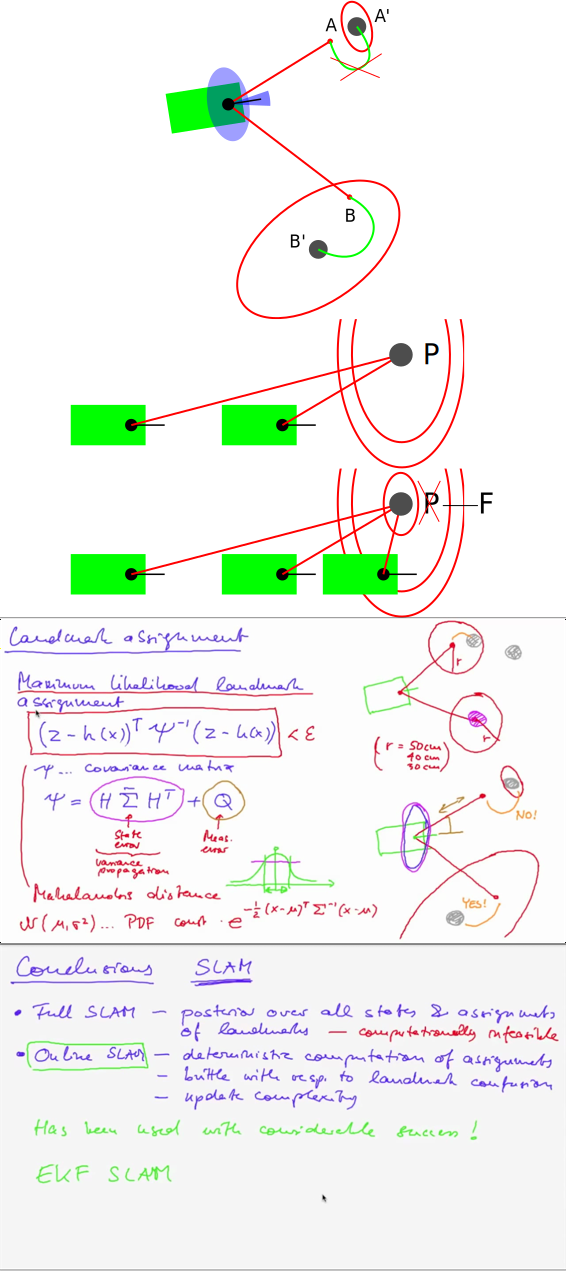
\includegraphics[scale=0.95]{../FIGURES/fig52}
\end{figure}

\begin{align*}
\vec{z}_{1t} \, = \, \begin{pmatrix}D_{1t}\\ \phi_{1t}\end{pmatrix}, ~ \vec{z}_{2t} \, = \, \begin{pmatrix}D_{2t}\\ \phi_{2t}\end{pmatrix}, ~ \vec{z}_{3t} \, = \, \begin{pmatrix}D_{3t}\\ \phi_{3t}\end{pmatrix}, ~ \vec{z}_{4t}  \, = \, \begin{pmatrix}D_{4t}\\ \phi_{4t}\end{pmatrix}
\end{align*}

I called \emph{world landmark} to a landmark that it's placed in a
specific position in the world that the algorithm knows since the
beginning of its execution.

The notation to reference in a generic way the position of any landmark
is:

\begin{align*}
\vec{p}_W\,=\,\begin{pmatrix}
x_W\\
y_W
\end{pmatrix}
\end{align*}The notation to reference to the position of the landmark number $j$
is:

\begin{align*}
{\vec{p}_W}_j\,=\,\begin{pmatrix}
{x_W}_j\\
{x_W}_j
\end{pmatrix}
\end{align*}

where $j\,=\,1,\,\ldots,\,N_w$.

The first task that the algorithm has to accomplish is to match each
detected landmark with a world landmark. These matches among the detected
landmarks and the world landmarks are based on the proximity among
them. 

The algorithm calculates the global coordinates of each detected landmark
using the robot's predicted pose, $\vec{\overline{\mu}}_t$, computed
in the predicted step, and each term $\vec{z}_{it}$.

The global coordinates of each detected landmark are:

\begin{align*}
x_{i} \,&=\, \overline{\mu}_{x_{lt}}\,+\,D_{it}\,\cos\left(\overline{\mu}_{\theta_t} \,+\, \phi_{it}\right)\,=\\
&=\,\overline{\mu}_{x_t} \,+\, sd\,\cos\left(\overline{\mu}_{\theta_t}\right) \,+\, D_{it}\,\cos\left(\overline{\mu}_{\theta_t} \,+\, \phi_{it}\right)\\
y_{i} \,&=\,\overline{\mu}_{y_{lt}}\,+\, D_{it}\,\sin\left(\overline{\mu}_{\theta_t} \,+\, \phi_{it}\right)\,=\\
&=\,\overline{\mu}_{y_t} \,+\, sd\,\sin\left(\overline{\mu}_{\theta_t}\right) \,+\, D_{it}\,\sin\left(\overline{\mu}_{\theta_t} \,+\, \phi_{it}\right)
\end{align*}

where $i\,=\, 1,\, 2,\, \ldots,\, N_s$.

The next step for the algorithm is to match each detected landmark
with the nearest world landmark. This task is possible since the algorithm
now knows the global coordinates of each detected landmark and each
world landmark. Let's suppose, that the algorithm has matched detected
landmark number 1 with world landmark number 2, detected landmark
number 2 with world landmark number 7, detected landmark number 3
with world landmark number 5 and detected landmark number 4 with world
landmark number 1.

\begin{align*}
\left(i\,=\,1,\,j\,=\,2\right),\,\left(i\,=\,2,\,j\,=\,7\right),\,\left(i\,=\,3,\,j\,=\,5\right),\,\left(i\,=\,4,\,j\,=\,1\right)\\
\end{align*}

If the distance from a detected landmark to its matched world landmark
is bigger than a maximum threshold, $\epsilon$, then this pair of
detected landmark-world landmark is rejected. 

\begin{align*}
\sqrt{\left(x_i\,-\,{x_W}_j\right)^2\,+\,\left(y_i\,-\,{y_W}_j\right)^2}\,&\leq\,\epsilon~\longrightarrow~\text{match accepted}\\[10pt]
\sqrt{\left(x_i\,-\,{x_W}_j\right)^2\,+\,\left(y_i\,-\,{y_W}_j\right)^2}\,&>\,\epsilon~\longrightarrow~\text{match rejected}
\end{align*}

Let's suppose that the second match in this example is rejected since
it doesn't satisfy the threshold condition. Therefore, the resulting
matches are:

\begin{align*}
\left(i\,=\,1,\,j\,=\,2\right),\,\left(i\,=\,3,\,j\,=\,5\right),\,\left(i\,=\,4,\,j\,=\,1\right)\\
\end{align*}

Before continuing it's necessary to define the concept of the expected
measurement. The term $\vec{\hat{z}}_t$ is called expected measurement.
The expected measurement to a world landmark is comprised by the distance
from the laser scanner to a world landmark, $\hat{D}_t$, and the
angle defined between the laser scanner's longitudinal axis and the
straight line that joints the laser scanner with the world landmark.

\begin{gather*}
\vec{\hat{z}}_t \,=\, h\left(\vec{x}_t,\,\vec{p}_W\right)\,=\,\begin{pmatrix*}[l]
\hat{D}_t\,=\,h_1\left(\vec{x}_{t},\,\vec{p}_W\right)\,=\,\sqrt{\left(x_W \,-\, x_{lt}\right)^2 \,+\, \left(y_W \,-\, y_{lt}\right)^2}\\[10pt]
\hat{\phi}_t\,=\,h_2\left(\vec{x}_{t},\,\vec{p}_W\right)\,=\,\arctan\left(\dfrac{y_W \,-\, y_{lt}}{x_W \,-\, x_{lt}}  \right) \,-\, \theta_t
\end{pmatrix*}\\[10pt]
\begin{pmatrix*}[l]
x_{lt}\,=\,x_t\,+\,sd\,\cos\left(\theta_t\right)\\[5pt]
y_{lt}\,=\,y_t\,+\,sd\,\sin\left(\theta_t\right)
\end{pmatrix*}\\[10pt]
\end{gather*}

The value $\vec{\hat{z}}_{jt}$ indicates the expected measurement
between the scanner laser's predicted position, $\vec{\overline{\mu}}_{lt}$,
and the position of the landmark number $j,\,{\vec{p}_W}_j$:

\begin{gather*}
\vec{\hat{z}}_{jt}\,=\,h\left(\vec{\overline{\mu}}_t,\,{\vec{p}_W}_j\right)\\
\begin{pmatrix*}[l]
\hat{D}_{jt}\,=\,h_1\left(\vec{\overline{\mu}}_t,\,{\vec{p}_W}_j\right)\,=\,\sqrt{\left({x_W}_j \,-\, \overline{\mu}_{x_{lt}}\right)^2 \,+\, \left({y_W}_j \,-\, \overline{\mu}_{y_{lt}}\right)^2}\\[10pt]
\hat{\phi}_{jt}\,=\,h_2\left(\vec{\overline{\mu}}_t,\,{\vec{p}_W}_j\right)\,=\,\arctan\left(\dfrac{{y_W}_j \,-\,\overline{\mu}_{y_{lt}}}{{x_W}_j\,-\,\overline{\mu}_{x_{lt}}}  \right) \,-\, \overline{\mu}_{\theta_t}
\end{pmatrix*}\\
\end{gather*}

\begin{figure}[H]
\centering\includegraphics[scale=0.95]{../FIGURES/fig50}
\end{figure}

Then for each world landmark successfully matched to a detected landmark
the algorithm computes the distance from the laser scanner's predicted
pose to that world landmark, $\hat{D}_{jt}$, and the angle defined
between the laser scanner's predicted longitudinal axis and the imaginary
line that joints the laser scanner's predicted position with that
world landmark, $\hat{\phi}_{jt}$. These computations are carried
out with the function $h\left(\vec{x}_t,\,\vec{p}_W\right)$. Therefore
the algorithm computes:

\begin{align*}
\vec{\hat{z}}_{2t}\,=\,\begin{pmatrix}\hat{D}_{2t}\\ \hat{\phi}_{2t}\end{pmatrix}\,=\,h\left(\overline{\mu}_t,\,{\vec{p}_W}_2\right)\\[10pt]
\vec{\hat{z}}_{5t}\,=\,\begin{pmatrix}\hat{D}_{5t}\\ \hat{\phi}_{5t}\end{pmatrix}\,=\,h\left(\overline{\mu}_t,\,{\vec{p}_W}_5\right)\\[10pt]
\vec{\hat{z}}_{1t}\,=\,\begin{pmatrix}\hat{D}_{1t}\\ \hat{\phi}_{1t}\end{pmatrix}\,=\,h\left(\overline{\mu}_t,\,{\vec{p}_W}_1\right)\\
\end{align*}

So, at this moment the algorithm has ended with the matching between
detected landmarks and world landmarks.

\begin{align*}
\left(\vec{z}_{1t},\, \vec{\hat{z}}_{2t}\right),\, \left(\vec{z}_{3t},\, \vec{\hat{z}}_{5t}\right),\, \left(\vec{z}_{4t},\, \vec{\hat{z}}_{1t}\right)
\end{align*}

\begin{align*}
\vec{z}_{1t} \, = \, \begin{pmatrix}D_{1t}\\ \phi_{1t}\end{pmatrix}, ~ \vec{z}_{3t} \, = \, \begin{pmatrix}D_{3t}\\ \phi_{3t}\end{pmatrix}, ~ \vec{z}_{4t}  \, = \, \begin{pmatrix}D_{4t}\\ \phi_{4t}\end{pmatrix}\\[10pt]
\vec{\hat{z}}_{2t} \, = \, \begin{pmatrix}\hat{D}_{2t}\\ \hat{\phi}_{2t}\end{pmatrix}, ~ \vec{\hat{z}}_{5t} \, = \, \begin{pmatrix}\hat{D}_{5t}\\ \hat{\phi}_{5t}\end{pmatrix}, ~ \vec{\hat{z}}_{1t}  \, = \, \begin{pmatrix}\hat{D}_{1t}\\ \hat{\phi}_{4t}\end{pmatrix}
\end{align*}

For each one of the previous matches the algorithm performs a correction
step. All these correction steps are carried out in a row, one after
the other. In the example there are three matches, so there are three
correction steps in a row. In each correction step the algorithm computes
the terms $H_t,\, K_t,\, \vec{\mu}_t$ and $\Sigma_t$.

The term $H_t$ is the jacobian matrix of the funcion $h\left(\vec{x}_t,\vec{p}_W\right)$
with respect to $\vec{x}_t$.

\begin{align*}
H_t \,=\, \dfrac{\partial h\left(\vec{x}_t,\,\vec{p}_W\right)}{\partial \vec{x}_t}
\,=\, \begin{pmatrix}\dfrac{\partial h_1}{\partial x_t} & \dfrac{\partial h_1}{\partial y_t} & \dfrac{\partial h_1}{\partial \theta_t}\\[10pt]
\dfrac{\partial h_2}{\partial x_t} & \dfrac{\partial h_2}{\partial y_t} & \dfrac{\partial h_2}{\partial \theta_t}
\end{pmatrix}
\end{align*}

Let's give a shorter name to some terms that are going to appear immediately:

\begin{gather*}
{\Delta x}_t\,\triangleq\,\left(x_W \,-\, x_{lt}\right)\\
{\Delta y}_t\,\triangleq\,\left(y_W \,-\, y_{lt}\right) \\
q_t\,\triangleq\, \left(x_W \,-\, x_{lt}\right)^2 \,+\, \left(y_W \,-\, y_{lt}\right)^2
\end{gather*}
\begin{align*}
\dfrac{\partial h_1}{\partial x_t} \,&=\, -\,\left(\dfrac{x_W \,-\, x_{lt}}{\sqrt{q_t}}\right) \,=\, -\,\dfrac{{\Delta x}_t}{\sqrt{q_t}}\\
\dfrac{\partial h_1}{\partial y_t} \,&=\, -\,\left(\dfrac{y_W \,-\, y_{lt}}{\sqrt{q_t}}\right) \,=\, -\,\dfrac{{\Delta y}_t}{\sqrt{q_t}}\\
\dfrac{\partial h_1}{\partial \theta_t} \,&=\, \dfrac{1}{2\,\sqrt{q_t}}\left(2\,{\Delta x}_t\,sd\,\sin\left(\theta_t\right) \,-\, 2\,{\Delta y}_t\,sd\,\cos\left(\theta_t\right)\right) \,=\\
&=\, \dfrac{sd}{\sqrt{q_t}}\,\left({\Delta x}_t\,\sin\left(\theta_t\right) \,-\, {\Delta y}_t\,\cos\left(\theta_t\right)\right)\\
\dfrac{\partial h_2}{\partial x_t} \,&=\, \dfrac{{\Delta y}_t}{q_t}\\
\dfrac{\partial h_2}{\partial y_t} \,&=\, -\,\dfrac{{\Delta x}_t}{q_t}\\
\dfrac{\partial h_2}{\partial \theta_t} \,&=\,-\,\dfrac{sd}{q_t}\,\left({\Delta x}_t\,\cos\left(\theta_t\right) \, + \, {\Delta y}_t\,\sin\left(\theta_t\right)\right) \,-\, 1
\end{align*}

In the first correction step the terms $\vec{\overline{\mu}}_t$ and
$\overline{\Sigma}_t$, computed in the predicted step, are used to
compute the terms $H_t,\, K_t,\, \vec{\mu}_t$ and $\Sigma_t$. If
there is more than one correction step, from the second correction
step onwards the results obtained at the end of the previous correction
step are feed into the current correction step that is about to star.
Therefore, It can be said that at the end of each intermediate correction
step the algorithm gives a partial corrected result. Only at the end
of the last correction step there is a definitive corrected result,
$\mu_t$ and $\Sigma_t$.

Continuing with our example, because of the algorithm could only match
three of those detected landmarks with world landmarks only three
correction steps are performed, one after the other, i.e, in a row,
using a \texttt{for} loop, even though four landmarks were detected
in the scan.

\mathleft

\begin{align*}
\vec{\mu}_t\,=\,\vec{\overline{\mu}}_t\\
\Sigma_t\,=\,\overline{\Sigma}_t
\end{align*}
\mathcenter

$\texttt{for } k\,=\,1\texttt{ to }N_{\texttt{matches}}:$

\begin{gather*}
H_t\left(\vec{\mu}_t,\,{\vec{p}_W}_j^{\,\left(\texttt{match k}\right)}\right)\\
K_t \,=\, \Sigma_t \,\cdot\, H_t^T \,\cdot\, \left(H_t \,\cdot \, \Sigma_t \,\cdot\, H_t^T \,+\, Q\right)^{-1}\\
\vec{\mu}_t \,=\, \vec{\mu}_t \, + \, K_t \,\cdot\, \left(\vec{z}_{it}^{\,\left(\texttt{match k}\right)}\,-\, \vec{\hat{z}}_{jt}^{\,\left(\texttt{match k}\right)}\right)\\
\Sigma_t \,=\, \left(I \,-\, K_t \,\cdot\, H_t\right)\,\cdot\,\Sigma_t
\end{gather*}

The term $\vec{z}_{it}^{\,\left(\texttt{match k}\right)}\,-\, \vec{\hat{z}}_{jt}^{\,\left(\texttt{match k}\right)}$
is called \textbf{innovation.}

The term $Q$ is the measurement covariance matrix, defined as:

\begin{align*}
Q \,=\, \begin{pmatrix}\sigma_D^2 & 0\\ 0 & \sigma_\phi^2\end{pmatrix}
\end{align*}

and appears in the probability density function:

\begin{align*}
p\left(\vec{z}_t \, \mid \, \vec{x}_t\right) \,=\, \mathcal{N}\left(\vec{\hat{z}}_t,\, Q\right)
\end{align*}

The first interesting thing that can be observed in the matrix $Q$
is that it doesn't depend on the time, subscript $t$, therefore,
it's a constant matrix. The second thing I observe is that the matrix
$Q$ is diagonal, so it means that the random variables $D_t$ and
$\phi_t$ are uncorrelated.\\

\textbf{A note about angles:}

Sometimes it's necessary to subtract two angles and a bit of attention
has to be paid in order to prevent mistakes when computing the difference.
For example, when the algorithm computes the innovation it has to
subtract the term $\vec{\hat{z}}_t$ from the term $\vec{z}_t$. In
this operation there is involved a subtraction of two angles.

\begin{align*}
\vec{z}_t \,-\, \vec{\hat{z}}_t \,=\, \begin{pmatrix}D_t \,-\, \hat{D}_t\\ \phi_t \,-\, \hat{\phi}_t\end{pmatrix}
\end{align*}

Let's suppose that:

\begin{align*}
\phi_t \,&=\, +\,180^{\circ} \,-\, \delta\\
\hat{\phi}_t \,&=\, -\,180^{\circ} \,+\, \epsilon
\end{align*}

and the angles $\delta$ and $\epsilon$ are contained in the first
quadrant, i.e, $0^{\circ}\,\leq\,\delta\,\leq\,90^{\circ}$ and $0^{\circ}\,\leq\,\epsilon\,\leq\,90^{\circ}$.
Therefore, $\phi_t$ is necessarily located in the second quadrant,
$90^{\circ}\,\leq\,\phi_t\,\leq\,180^{\circ}$, and $\hat{\phi}_t$
is necessarily located in the third quadrant, $-\,180^{\circ}\,\leq\,\hat{\phi}_t\,\leq\,-\,90^{\circ}$. 

\begin{gather*}
\phi_t \,-\, \hat{\phi}_t \,=\, 180^{\circ} \,-\, \delta \,-\,\left(-\,180^{\circ} \,+\, \epsilon\right) \,=\, 360^{\circ} \,-\,\left(\delta \,+\, \epsilon\right)\\
180^{\circ}\,\leq\,\phi_t \,-\, \hat{\phi}_t\,\leq\,360^{\circ}
\end{gather*}

If you are working with angles in the range $\left[-\,180^{\circ},\, +\,180^{\circ}\right]$
the angle $\phi_t \,-\, \hat{\phi}_t$, which is in the range $\left[+\,180^{\circ},\,+\,360^{\circ}\right]$,
is not admissible. The angle that you would like is $-\,\left(\delta\,+\,\epsilon\right)$,
which is in the range $\left[-\,180^{\circ},\, +\,180^{\circ}\right]$.
So, every time you work with angles that must belong to the range
$\left[-\,180^{\circ},\, +\,180^{\circ}\right]$ you must do the following
correction:

\begin{align*}
\left(\left(\left(\phi_t \,-\, \hat{\phi}_t\right) \,+\, \pi\right)\bmod\,2\pi\right) \,-\, \pi
\end{align*}

\newpage

Example:

\begin{align*}
\delta \,&=\, 30^{\circ}\\
\epsilon \,&=\, 45^{\circ}\\
\phi_t \,&=\, +\,180^{\circ} \,-\, \delta \,=\, +\,150^{\circ}\\
\hat{\phi}_t \,&=\, -\,180^{\circ} \,+\, \epsilon \,=\, -135^{\circ}\\
\phi_t \,-\, \hat{\phi}_t \,&=\, 150^{\circ} \,-\,\left(-\,135^{\circ}\right) \,=\,150^{\circ} \,+\,135^{\circ}\,=\,285^{\circ}\\
\left(\phi_t \,-\, \hat{\phi}_t\right) \,+\, 180^{\circ} \,&=\, 285^{\circ}\,+\,180^{\circ}\,=\,465^{\circ}\\
\left(\left(\phi_t \,-\, \hat{\phi}_t\right) \,+\, 180^{\circ}\right)\bmod\,360^{\circ} \,&=\,465^{\circ}\bmod 360^{\circ}\,=\,105^{\circ}\\
\left(\left(\left(\phi_t \,-\, \hat{\phi}_t\right) \,+\, 180^{\circ}\right)\bmod\,360^{\circ}\right) \,-\, 180^{\circ} \,&=\, 105^{\circ} \,-\, 180^{\circ} \,=\, -\,75^{\circ} \,=\, -\,\left(\delta\,+\,\epsilon\right)
\end{align*}

\begin{figure}[H]
\centering\includegraphics[scale=0.95]{../FIGURES/fig54}
\end{figure}

Note:

\begin{align*}
\vec{\overline{\mu}}_t \,&= \, \begin{pmatrix}
\overline{\mu}_{x_t}\\
\overline{\mu}_{y_t}\\
\overline{\mu}_{\theta_t}
\end{pmatrix} \,=\, \begin{pmatrix}
\widetilde{x}_t\\
\widetilde{y}_t\\
\widetilde{\theta}_t
\end{pmatrix} \,=\, \vec{\widetilde{x}}_t \\[10pt]
\vec{\mu}_t \,&= \, \begin{pmatrix}
\mu_{x_t}\\
\mu_{y_t}\\
\mu_{\theta_t}
\end{pmatrix} \,=\, \begin{pmatrix}
\widehat{x}_t\\
\widehat{y}_t\\
\widehat{\theta}_t
\end{pmatrix} \,=\, \vec{\widehat{x}}_t
\end{align*}

\begin{landscape}

\begin{figure}[H]
\centering\includegraphics[scale=0.95]{../FIGURES/fig56}
\end{figure}

\end{landscape}
\end{document}
